\documentclass[12pt,a4paper,twoside]{report}

%==========================================================
% PACKAGES ET CONFIGURATION
%==========================================================
\usepackage[backend=biber, style=apa]{biblatex}
\addbibresource{references.bib}
\usepackage[utf8]{inputenc}
\usepackage[T1]{fontenc}
\usepackage[french]{babel}
\usepackage{csquotes}
\usepackage{mathpazo}
\usepackage[scaled=0.92]{helvet}
\usepackage{courier}
\usepackage{microtype}
\usepackage{geometry}
\usepackage[dvipsnames,table]{xcolor}
\usepackage{graphicx}
\usepackage{float}
\usepackage{booktabs}
\usepackage{tabularx}
\usepackage{longtable}
\usepackage{array}
\usepackage{enumitem}
\usepackage{fancyhdr}
\usepackage{titlesec}
\usepackage{titletoc}
\usepackage{tcolorbox}
\usepackage{tikz}
\usepackage{listings}
\usepackage{caption}
\usepackage{subcaption}
\usepackage{hyperref}
\usepackage{iftex}
\usepackage{amssymb}
\usepackage{textcomp}
\usepackage{multirow}
\usepackage{amsmath}

\tcbuselibrary{skins}
\usetikzlibrary{positioning,arrows.meta}

%==========================================================
% MISE EN PAGE
%==========================================================
\geometry{
  a4paper,
  top=2.5cm,
  bottom=2.7cm,
  inner=3cm,
  outer=2.2cm,
  headheight=25pt,
  includehead
}

%==========================================================
% COULEURS
%==========================================================
\definecolor{PrimaryRed}{RGB}{72,61,139}
\definecolor{DarkSlate}{RGB}{38,42,52}
\definecolor{MidGray}{RGB}{96,102,112}
\definecolor{LightGray}{RGB}{246,247,250}
\definecolor{SoftRed}{RGB}{255,247,246}
\definecolor{AccentBlue}{RGB}{48,104,178}
\definecolor{TableHeader}{RGB}{48,52,64}
\colorlet{primary}{PrimaryRed}

%==========================================================
% HYPERLIENS
%==========================================================
\hypersetup{
  colorlinks=true,
  linkcolor=PrimaryRed,
  urlcolor=AccentBlue,
  citecolor=PrimaryRed,
  pdftitle={ALO pour le PFSP -- Analyse Comparative},
  pdfauthor={El Gharib Mahmoud}
}

%==========================================================
% PARAGRAPHES
%==========================================================
\setlength{\parindent}{15pt}
\setlength{\parskip}{0pt}
\linespread{1.08}

%==========================================================
% EN-TETES ET PIEDS DE PAGE
%==========================================================
\pagestyle{fancy}
\fancyhf{}
\fancyhead[LE]{\small\color{MidGray}\leftmark}
\fancyhead[RO]{\small\color{MidGray}\rightmark}
\fancyfoot[C]{\small\color{MidGray}\thepage}
\renewcommand{\headrulewidth}{0.4pt}
\renewcommand{\headrule}{\hbox to\headwidth{\color{PrimaryRed}\leaders\hrule height \headrulewidth\hfill}}

%==========================================================
% FORMAT DES CHAPITRES
%==========================================================
\titleformat{\chapter}[display]
  {\normalfont\color{DarkSlate}}
  {%
    \begin{tikzpicture}[baseline]
      \node[
        fill=PrimaryRed,
        text=white,
        rounded corners=2pt,
        inner xsep=12pt,
        minimum height=0.72cm,
        font=\Large\bfseries
      ] {\chaptertitlename~\thechapter};
    \end{tikzpicture}
  }
  {14pt}
  {\Huge\bfseries}
  [\vspace{6pt}{\color{PrimaryRed}\rule{\textwidth}{1.2pt}}]
\titlespacing*{\chapter}{0pt}{-12pt}{30pt}

%==========================================================
% FORMAT DES SECTIONS
%==========================================================
\titleformat{\section}
  {\normalfont\Large\bfseries\color{DarkSlate}}
  {\color{PrimaryRed}\thesection}{0.8em}{}
  [\vspace{-3pt}{\color{MidGray!35}\rule{\textwidth}{0.5pt}}]

\titleformat{\subsection}
  {\normalfont\large\bfseries\color{DarkSlate}}
  {\color{PrimaryRed}\thesubsection}{0.7em}{}

%==========================================================
% TABLE DES MATIÈRES
%==========================================================
\titlecontents{chapter}[0pt]
  {\vspace{7pt}\bfseries\color{DarkSlate}}
  {\contentslabel{2em}}{}
  {\hfill\color{PrimaryRed}\contentspage}

\titlecontents{section}[2em]
  {\vspace{2pt}\color{MidGray}}
  {\contentslabel{2.3em}}{}
  {\titlerule*[0.5pc]{.}\contentspage}

%==========================================================
% LISTES
%==========================================================
\setlist[itemize]{leftmargin=1.4em,itemsep=2pt,topsep=3pt}
\setlist[enumerate]{leftmargin=1.4em,itemsep=2pt,topsep=3pt}

%==========================================================
% LÉGENDES
%==========================================================
\captionsetup{
  labelfont={bf,color=PrimaryRed},
  textfont={small,color=DarkSlate},
  justification=centering
}

%==========================================================
% BOÎTES COLORÉES
%==========================================================
\tcbset{
  enhanced,
  boxrule=0.6pt,
  arc=3pt,
  left=8pt,
  right=8pt,
  top=7pt,
  bottom=7pt
}

\newtcolorbox{infobox}[1]{
  colback=SoftRed,
  colframe=PrimaryRed,
  title={#1},
  fonttitle=\bfseries,
  coltitle=white,
  colbacktitle=PrimaryRed
}

\newtcolorbox{resultbox}[1]{
  colback=LightGray,
  colframe=DarkSlate!35,
  title={#1},
  fonttitle=\bfseries,
  coltitle=DarkSlate,
  colbacktitle=white
}

%==========================================================
% CODE SOURCE
%==========================================================
\lstset{
  basicstyle=\footnotesize\ttfamily,
  keywordstyle=\color{AccentBlue}\bfseries,
  commentstyle=\color{MidGray}\itshape,
  stringstyle=\color{PrimaryRed},
  backgroundcolor=\color{LightGray},
  frame=single,
  rulecolor=\color{MidGray!45},
  breaklines=true,
  showstringspaces=false,
  columns=fullflexible,
  keepspaces=true
}

%==========================================================
% COMMANDE PERSONNALISÉE
%==========================================================
\newcommand{\projectname}{ALO pour le PFSP}

\begin{document}

%==========================================================
% PAGE DE GARDE
%==========================================================
\begin{titlepage}
  \thispagestyle{empty}
  \enlargethispage{1.4cm}
  
  \noindent
  \begin{minipage}[c]{0.30\linewidth}
    \raggedright
    \includegraphics[width=3.25cm]{logo1.png}
  \end{minipage}
  \hfill
  \begin{minipage}[c]{0.38\linewidth}
    \centering
    {\small\textbf{Université Abdelmalek Essaâdi}}\\
    {\scriptsize Faculté des Sciences et Techniques -- Tanger}
  \end{minipage}
  \hfill
  \begin{minipage}[c]{0.30\linewidth}
    \raggedleft
    \includegraphics[width=3.25cm]{logo2.png}
  \end{minipage}

  \vspace{0.45cm}

  \begin{center}
    {\normalsize\bfseries MASTER SCIENCES ET TECHNIQUES}\\[0.1cm]
    {\normalsize\bfseries INTELLIGENCE ARTIFICIELLE ET SCIENCES DES DONNÉES}\\[0.35cm]

    \begin{tcolorbox}[
      colback=PrimaryRed!5,
      colframe=PrimaryRed,
      width=0.78\linewidth,
      arc=4pt,
      boxrule=0.9pt,
      left=8pt,
      right=8pt,
      top=6pt,
      bottom=6pt
    ]
      \centering
      {\large\textbf{Module : Métaheuristiques}}
    \end{tcolorbox}

    \vspace{0.55cm}

    \begin{tcolorbox}[
      colback=white,
      colframe=PrimaryRed,
      width=0.90\linewidth,
      arc=6pt,
      boxrule=1.2pt,
      left=14pt,
      right=14pt,
      top=13pt,
      bottom=13pt,
      borderline west={3pt}{0pt}{PrimaryRed}
    ]
      \centering
      {\Huge\bfseries\textcolor{PrimaryRed}{Rapport}}\\[0.35cm]
      {\LARGE\bfseries\textcolor{DarkSlate}{Ant Lion Optimizer pour le}\\[0.1cm]
       \LARGE\bfseries\textcolor{DarkSlate}{Flow Shop Scheduling}}\\[0.22cm]
      {\large\bfseries Analyse Comparative sur Instances Taillard}\\[0.35cm]
      {\normalsize Implémentation et évaluation statistique de l'ALO adapté au PFSP avec Random Keys.}
    \end{tcolorbox}
  \end{center}

  \vspace{0.45cm}

  \begin{tcolorbox}[
    colback=LightGray,
    colframe=MidGray!45,
    width=\linewidth,
    arc=4pt,
    boxrule=0.6pt,
    left=12pt,
    right=12pt,
    top=8pt,
    bottom=8pt
  ]
    \noindent
    \begin{minipage}[t]{0.48\linewidth}
      \textbf{\textcolor{PrimaryRed}{Encadré par :}}\\[0.15cm]
      Pr.\ Khalid Jebari
    \end{minipage}
    \hfill
    \begin{minipage}[t]{0.48\linewidth}
      \raggedleft
      \textbf{\textcolor{PrimaryRed}{Réalisé par :}}\\[0.15cm]
      \textit{El Gharib Mahmoud}
    \end{minipage}
  \end{tcolorbox}

  \vspace{0.15cm}
  \noindent
  \textbf{\textcolor{PrimaryRed}{Dépôt :}} \href{https://github.com/mahmoud-ath/ALO_FLOWSHOP_METHAHEURISTIQUE}{https://github.com/mahmoud-ath/ALO_FLOWSHOP_METHAHEURISTIQUE}

  \vspace{0.35cm}

  \begin{center}
    \textcolor{PrimaryRed}{\rule{0.45\linewidth}{0.8pt}}\\[0.25cm]
    {\large\bfseries Année Universitaire 2025--2026}
  \end{center}
\end{titlepage}

%==========================================================
% FRONT MATTER
%==========================================================
\newpage
\pagenumbering{roman}
\setcounter{page}{1}

\tableofcontents
\newpage

\listoffigures
\newpage

\listoftables
\newpage

%==========================================================
% MAIN CONTENT
%==========================================================
\pagenumbering{arabic}
\setcounter{page}{1}

%==========================================================
% RÉSUMÉ
%==========================================================
\chapter*{Résumé}
\addcontentsline{toc}{chapter}{Résumé}

Ce rapport présente une implémentation et une évaluation approfondie de l'\textbf{Ant Lion Optimizer (ALO)} \cite{mirjalili2015} adapté au \textbf{Permutation Flow Shop Scheduling Problem (PFSP)}. L'adaptation repose sur le mécanisme des \textbf{Random Keys} pour convertir les positions continues de l'ALO en permutations valides de jobs. L'algorithme est comparé à un \textbf{Algorithme Génétique (GA)} avec crossover PMX et à une \textbf{Recherche Aléatoire (RS)} sur six instances Taillard de tailles variées (20 à 100 jobs, 5 à 20 machines). Chaque configuration est évaluée sur \textbf{30 exécutions indépendantes} avec analyse statistique incluant le test de rang signé de Wilcoxon. Les résultats montrent que l'ALO surpasse significativement la recherche aléatoire sur toutes les instances et rivalise avec le GA, obtenant le meilleur makespan sur 4 des 6 instances.

\vspace{0.4cm}
\noindent\textbf{Mots-clés :} Ant Lion Optimizer, Flow Shop Scheduling, Métaheuristique, Optimisation Combinatoire, Random Keys, Benchmarks Taillard

\begin{infobox}{Apport principal du projet}
Adaptation fidèle de l'ALO au PFSP avec évaluation statistique rigoureuse (30 runs $\times$ 3 algorithmes $\times$ 6 instances = 540 exécutions) incluant comparaison aux Best-Known Solutions (BKS) et tests de Wilcoxon.
\end{infobox}

%==========================================================
% CHAPITRE 1 : INTRODUCTION
%==========================================================
\chapter{Introduction générale}

\section{Contexte et problème traité}

Le \textbf{Permutation Flow Shop Scheduling Problem (PFSP)} est un problème d'optimisation combinatoire $\mathcal{NP}$-difficile classique où $n$ jobs doivent être traités sur $m$ machines dans le même ordre séquentiel. Chaque machine ne peut traiter qu'un seul job à la fois, et chaque job ne peut être traité que sur une seule machine à la fois.

L'\textbf{objectif} est de trouver une permutation $\pi = [\pi_1, \pi_2, \dots, \pi_n]$ qui \textbf{minimise le makespan} $C_{\max}$, c'est-à-dire le temps d'achèvement du dernier job sur la dernière machine.

Le makespan $C_{\max}$ est défini récursivement par :
\begin{align}
    C_{\pi_1,1} &= P_{\pi_1,1} \nonumber \\
    C_{\pi_j,1} &= C_{\pi_{j-1},1} + P_{\pi_j,1} \quad \forall j > 1 \\
    C_{\pi_1,k} &= C_{\pi_1,k-1} + P_{\pi_1,k} \quad \forall k > 1 \nonumber \\
    C_{\pi_j,k} &= \max(C_{\pi_j,k-1}, C_{\pi_{j-1},k}) + P_{\pi_j,k} \quad \forall j,k > 1 \nonumber
\end{align}
où $P_{j,k}$ est le temps de traitement du job $j$ sur la machine $k$.

\section{Ant Lion Optimizer (ALO)}

L'ALO, proposé par \textbf{Mirjalili (2015)} \cite{mirjalili2015}, est une métaheuristique d'optimisation inspirée du comportement de chasse des fourmilions (\textit{antlions}). L'algorithme maintient deux populations :
\begin{itemize}
    \item \textbf{Fourmis (\textit{ants})} --- agents explorateurs qui effectuent des marches aléatoires;
    \item \textbf{Fourmilions (\textit{antlions})} --- agents piégeurs qui représentent des solutions de haute qualité.
\end{itemize}

Le mécanisme de chasse comprend cinq étapes :
\begin{enumerate}
    \item \textbf{Marche aléatoire} --- exploration via somme cumulée de pas stochastiques;
    \item \textbf{Construction de pièges} --- sélection par roulette wheel pondérée par la fitness;
    \item \textbf{Rétrécissement adaptatif} --- contraction progressive des frontières de recherche;
    \item \textbf{Capture} --- remplacement d'un antlion par une fourmi plus performante;
    \item \textbf{Élitisme} --- préservation systématique du meilleur antlion.
\end{enumerate}

\section{Objectifs du projet}

\begin{itemize}
  \item Adapter l'ALO au PFSP via le mécanisme des Random Keys;
  \item Comparer l'ALO à un Algorithme Génétique (GA) et à une Recherche Aléatoire (RS);
  \item Évaluer les algorithmes sur plusieurs instances Taillard de tailles variées;
  \item Produire une analyse statistique rigoureuse incluant le test de Wilcoxon;
  \item Comparer les résultats aux Best-Known Solutions (BKS) de la littérature.
\end{itemize}

\section{Méthodologie}

La méthodologie adoptée comprend :
\begin{enumerate}
  \item Implémentation de l'ALO original (Mirjalili, 2015) avec adaptation Random Keys;
  \item Implémentation d'un GA de référence avec crossover PMX et mutation par échange;
  \item Définition d'un protocole expérimental : 30 runs indépendants par configuration;
  \item Exécution sur 6 instances Taillard (20 à 100 jobs, 5 à 20 machines);
  \item Analyse statistique : moyenne, écart-type, test de Wilcoxon, Gap\% par rapport au BKS.
\end{enumerate}

\begin{figure}[H]
\centering
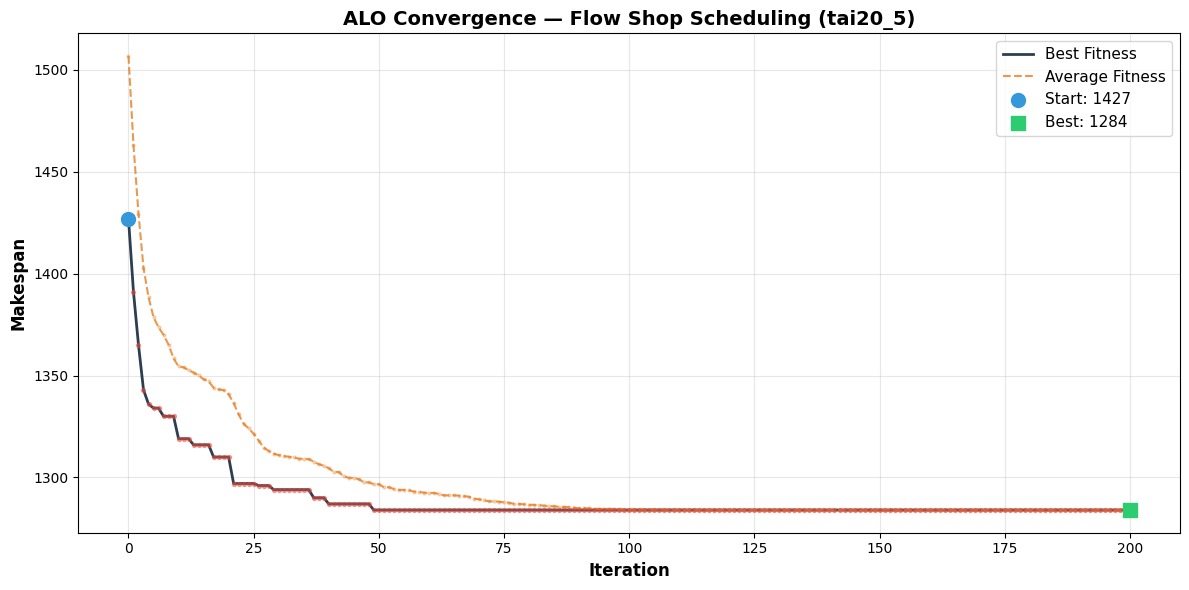
\includegraphics[width=0.85\textwidth]{figures/convergence_tai20_5.png}
\caption{Courbes de convergence --- Moyenne $\pm$ 1$\sigma$ sur 30 runs (tai20\_5).}
\label{fig:convergence}
\end{figure}

%==========================================================
% CHAPITRE 2 : ARCHITECTURE
%==========================================================
\chapter{Architecture de l'implémentation}

\section{Adaptation continue $\rightarrow$ permutation}

Le tableau~\ref{tab:adaptation} résume l'adaptation de l'ALO continu au PFSP.

\begin{table}[H]
\centering
\rowcolors{2}{LightGray}{white}
\caption{Adaptation de l'ALO continu au PFSP}
\label{tab:adaptation}
\begin{tabular}{>{\raggedright\arraybackslash}p{5cm} >{\raggedright\arraybackslash}p{8cm}}
\toprule
\rowcolor{TableHeader}
\color{white}ALO Original (Continu) & \color{white}ALO adapté au PFSP \\
\midrule
Vecteur position $\mathbf{x} \in \mathbb{R}^n$ & Vecteur position $\mathbf{x} \in \mathbb{R}^n$ (inchangé) \\
Fonction objectif $f(\mathbf{x})$ & Random Keys $\rightarrow$ Permutation $\pi$ $\rightarrow$ $C_{\max}(\pi)$ \\
\bottomrule
\end{tabular}
\end{table}

\begin{infobox}{Préservation de l'algorithme original}
Seule la fonction d'évaluation est modifiée. La totalité de la structure algorithmique --- marche aléatoire, roulette wheel, élite, remplacement, frontières adaptatives --- est \textbf{100\% conforme} à l'article original de Mirjalili \cite{mirjalili2015}.
\end{infobox}

\section{Pipeline algorithmique}

Le pipeline de l'ALO pour le PFSP est décrit ci-dessous :

\begin{lstlisting}
1. Initialiser populations (ants, antlions) uniformement dans [lb, ub]
2. Evaluer : continu -> argsort -> permutation -> makespan
3. Trier antlions par fitness. Elite = meilleur antlion.
4. Pour t = 1 a max_iter:
      Pour chaque fourmi i:
          a. Roulette wheel -> antlion cible
          b. Random walk autour de l'antlion
          c. Random walk autour de l'elite
          d. Nouvelle position = moyenne des 2 walks
      Clip aux frontieres [lb, ub]
      Evaluer toutes les fourmis
      Remplacer antlions si fourmis meilleures
      Mettre a jour l'elite
5. Retourner meilleure permutation + makespan
\end{lstlisting}

\section{Marche aléatoire}

La marche aléatoire constitue le c{\oe}ur de l'exploration :
\begin{equation}
X(t) = \left[0, \sum_{i=1}^{t} (2r(t_i)-1)\right]
\end{equation}
où $r(t) \sim \mathcal{U}(0,1)$ et :
\begin{equation}
2r(t)-1 = \begin{cases} +1 & \text{si } r(t) > 0.5 \\ -1 & \text{sinon} \end{cases}
\end{equation}

Le coefficient adaptatif $I$ contrôle le rétrécissement des frontières :
\begin{equation}
I = 
\begin{cases}
1 + 10 \cdot \frac{t}{T} & \text{si } t > 0.1T \\
1 + 10 \cdot \frac{t}{T} & \text{si } t > 0.5T \\
1 + 100 \cdot \frac{t}{T} & \text{si } t > 0.75T \\
1 + 1000 \cdot \frac{t}{T} & \text{si } t > 0.9T \\
1 + 10000 \cdot \frac{t}{T} & \text{si } t > 0.95T
\end{cases}
\end{equation}

Les frontières rétrécies centrées sur la position cible sont :
\begin{equation}
\text{lb}_t = \mathbf{p} + \frac{\text{lb}}{I}, \quad \text{ub}_t = \mathbf{p} + \frac{\text{ub}}{I}
\end{equation}

La normalisation min-max projette la marche dans $[\text{lb}_t, \text{ub}_t]$ :
\begin{equation}
X_{\text{norm}} = \frac{(X - a)(d - c)}{b - a} + c
\end{equation}

\section{Fonctions implémentées}

Le tableau~\ref{tab:composants} liste les composants de l'implémentation.

\begin{table}[H]
\centering
\rowcolors{2}{LightGray}{white}
\caption{Composants de l'implémentation ALO}
\label{tab:composants}
\begin{tabular}{>{\raggedright\arraybackslash}p{4.5cm} >{\raggedright\arraybackslash}p{6.5cm} >{\raggedright\arraybackslash}p{2.5cm}}
\toprule
\rowcolor{TableHeader}
\color{white}Fonction & \color{white}Description & \color{white}Mirjalili \\
\midrule
\texttt{calculate\_makespan()} & Calcule $C_{\max}$ pour une permutation & Nouveau (PFSP) \\
\texttt{continuous\_to\_permutation()} & Random Keys : argsort d'un vecteur continu & Nouveau (PFSP) \\
\texttt{initialize\_population()} & Initialisation uniforme dans $[lb, ub]$ & 100\% \\
\texttt{roulette\_wheel()} & Sélection proportionnelle inversée & 100\% \\
\texttt{random\_walk()} & Somme cumulée de $(2r>1)-1$, coefficient $I$ & 100\% \\
\texttt{clip\_population()} & Contrainte des positions dans $[lb, ub]$ & 100\% \\
\texttt{evaluate\_population()} & Continu $\rightarrow$ permutation $\rightarrow$ makespan & Adapté \\
\texttt{replace\_antlions()} & Remplacement si fourmi plus fitte & 100\% \\
\texttt{update\_elite()} & Mise à jour de l'élite & 100\% \\
\texttt{alo()} & Boucle principale complète & 100\% \\
\bottomrule
\end{tabular}
\end{table}

%==========================================================
% CHAPITRE 3 : PROTOCOLE
%==========================================================
\chapter{Protocole expérimental}

\section{Instances de test}

Six instances de la benchmark Taillard \cite{taillard1993} sont utilisées (tableau~\ref{tab:instances}).

\begin{table}[H]
\centering
\rowcolors{2}{LightGray}{white}
\caption{Instances Taillard utilisées}
\label{tab:instances}
\begin{tabular}{cccc}
\toprule
\rowcolor{TableHeader}
\color{white}Instance & \color{white}Jobs ($n$) & \color{white}Machines ($m$) & \color{white}BKS \\
\midrule
tai20\_5  & 20  & 5   & 1278 \\
tai20\_10 & 20  & 10  & 1582 \\
tai50\_5  & 50  & 5   & 2724 \\
tai50\_10 & 50  & 10  & 2995 \\
tai100\_10 & 100 & 10  & 5494 \\
tai100\_20 & 100 & 20  & 6208 \\
\bottomrule
\end{tabular}
\end{table}

\section{Paramètres des algorithmes}

Le tableau~\ref{tab:params} présente les paramètres d'exécution.

\begin{table}[H]
\centering
\rowcolors{2}{LightGray}{white}
\caption{Paramètres d'exécution}
\label{tab:params}
\begin{tabular}{lccc}
\toprule
\rowcolor{TableHeader}
\color{white}Paramètre & \color{white}ALO & \color{white}GA & \color{white}RS \\
\midrule
Taille population & 40 & 40 & --- \\
Itérations & 200 & 200 & --- \\
Domaine de recherche & $[-4, 4]$ & --- & --- \\
Échantillons & --- & --- & 5000 \\
Taux crossover & --- & 0.8 & --- \\
Taux mutation & --- & 0.1 & --- \\
Élitisme & --- & 2 & --- \\
Runs indépendants & \textbf{30} & \textbf{30} & \textbf{30} \\
Seeds & $run \times 100 + 42$ & $run \times 100 + 42$ & $run \times 100 + 42$ \\
\bottomrule
\end{tabular}
\end{table}

\section{Métriques d'évaluation}

Pour chaque algorithme sur chaque instance, nous calculons :
\begin{itemize}
    \item \textbf{Best} --- makespan minimum sur 30 runs;
    \item \textbf{Mean} --- moyenne arithmétique des 30 runs;
    \item \textbf{Worst} --- makespan maximum;
    \item \textbf{Std} --- écart-type (avec correction de Bessel, $n-1$);
    \item \textbf{Avg Time} --- temps d'exécution moyen (secondes);
    \item \textbf{Gap\%} --- $\dfrac{\text{Algorithme} - \text{BKS}}{\text{BKS}} \times 100$.
\end{itemize}

\section{Test statistique}

Le \textbf{test de Wilcoxon pour échantillons appariés} (test non-paramétrique) est utilisé pour comparer les paires d'algorithmes (RS vs GA, RS vs ALO, GA vs ALO) sur les 30 runs, avec un seuil de significativité $\alpha = 0.05$. Ce test est préféré au test $t$ de Student car il ne suppose pas la normalité des distributions.

%==========================================================
% CHAPITRE 4 : RÉSULTATS
%==========================================================
\chapter{Résultats expérimentaux}

\section{Analyse sur l'instance tai20\_5}

Le tableau~\ref{tab:stats_tai20_5} présente les statistiques descriptives pour l'instance tai20\_5.

\begin{table}[H]
\centering
\rowcolors{2}{LightGray}{white}
\caption{Statistiques descriptives --- tai20\_5 (30 runs)}
\label{tab:stats_tai20_5}
\begin{tabular}{lccccc}
\toprule
\rowcolor{TableHeader}
\color{white}Algorithme & \color{white}Best & \color{white}Mean & \color{white}Worst & \color{white}Std & \color{white}Temps (s) \\
\midrule
Random Search    & 1327 & 1353.1 & 1376 & 9.59  & 0.20 \\
Genetic Algorithm & 1278 & 1304.0 & 1331 & 15.81 & 0.51 \\
\textbf{ALO}  & \textbf{1273} & \textbf{1291.0} & \textbf{1320} & \textbf{12.48} & \textbf{6.24} \\
\bottomrule
\end{tabular}
\end{table}

ALO obtient le meilleur makespan (1273, soit \textbf{-0.39\% sous le BKS}), la meilleure moyenne (1291.0), et est statistiquement supérieur au GA ($p = 0.0055$, test de Wilcoxon). Le GA est plus rapide (0.51 s contre 6.24 s), ce qui reflète la complexité des marches aléatoires multidimensionnelles de l'ALO.

\begin{figure}[H]
\centering
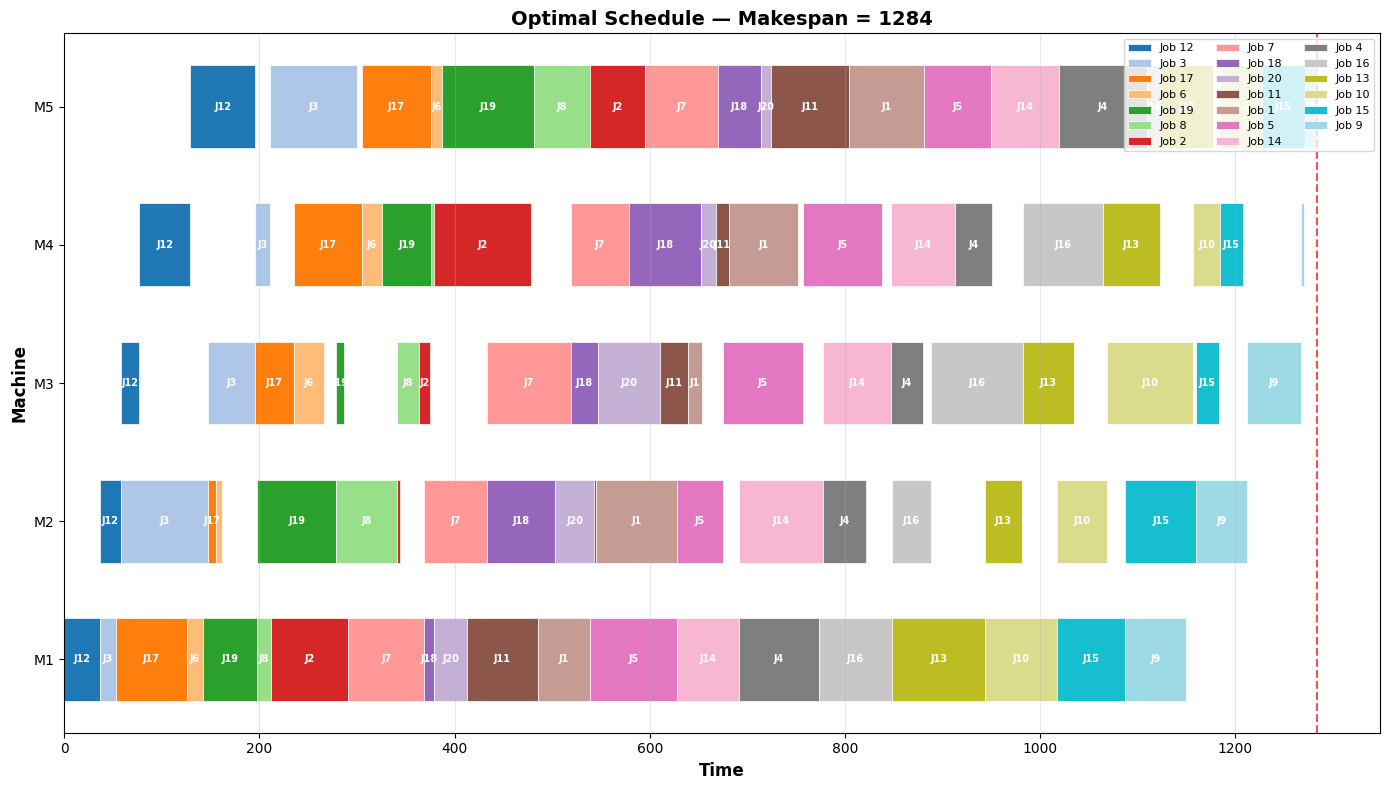
\includegraphics[width=0.82\textwidth]{figures/barchart_tai20_5.png}
\caption{Diagrammes en barres --- Best makespan, moyenne $\pm$ 1$\sigma$, et temps d'exécution (tai20\_5).}
\label{fig:barchart}
\end{figure}

\begin{figure}[H]
\centering
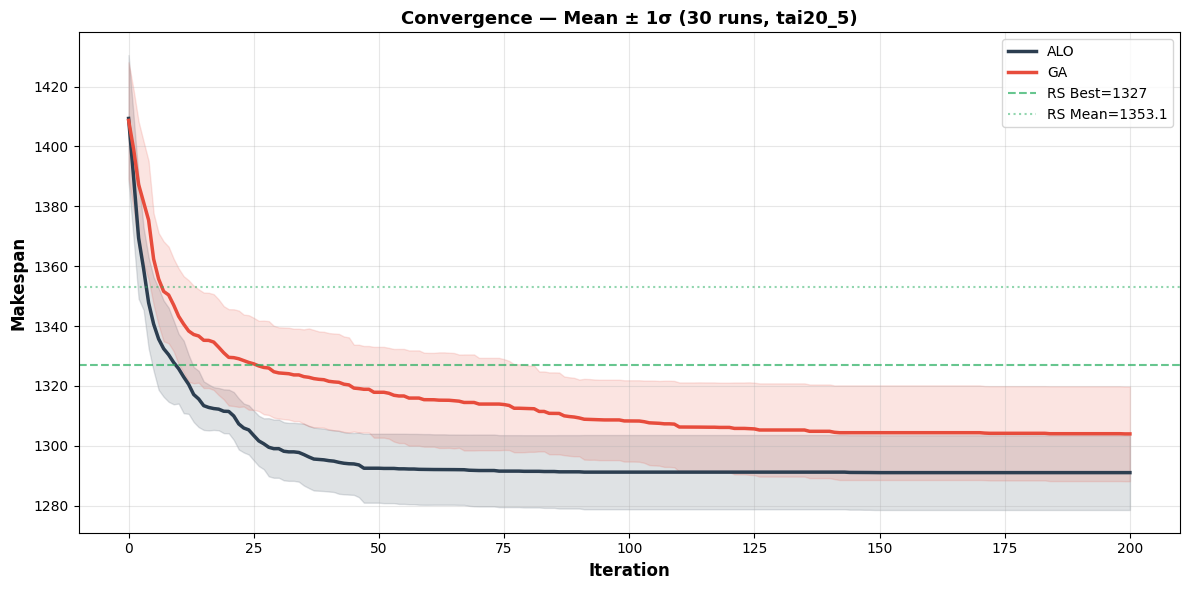
\includegraphics[width=0.72\textwidth]{figures/boxplot_tai20_5.png}
\caption{Box plot --- Distribution des makespans sur 30 runs (tai20\_5).}
\label{fig:boxplot}
\end{figure}

\section{Grille de comparaison complète}

Le tableau~\ref{tab:grid} présente la grille complète des résultats avec le Gap\% par rapport au BKS.

\begin{table}[H]
\centering
\rowcolors{2}{LightGray}{white}
\caption{Grille de comparaison complète avec BKS Gap\%}
\label{tab:grid}
\small
\begin{tabular}{lccccccl}
\toprule
\rowcolor{TableHeader}
\color{white}Instance & \color{white}Algo. & \color{white}Best & \color{white}Mean & \color{white}Std & \color{white}T(s) & \color{white}BKS & \color{white}Gap\% \\
\midrule
\multirow{3}{*}{tai20\_5}
 & RS  & 1327 & 1353.1 & 9.59  & 0.23 & \multirow{3}{*}{1278} & 3.83 \\
 & GA  & 1278 & 1304.0 & 15.81 & 0.51 & & 0.00 \\
 & \textbf{ALO} & \textbf{1273} & \textbf{1291.0} & \textbf{12.48} & \textbf{6.23} & & \textbf{-0.39} \\
\midrule
\multirow{3}{*}{tai20\_10}
 & RS  & 1834 & 1880.6 & 16.09 & 0.37 & \multirow{3}{*}{1582} & 15.93 \\
 & \textbf{GA} & \textbf{1745} & \textbf{1780.4} & \textbf{18.39} & \textbf{0.78} & & \textbf{10.30} \\
 & ALO & 1750 & 1767.1 & 14.63 & 6.52 & & 10.62 \\
\midrule
\multirow{3}{*}{tai50\_5}
 & RS  & 2941 & 2990.2 & 18.02 & 0.46 & \multirow{3}{*}{2724} & 7.97 \\
 & \textbf{GA} & \textbf{2838} & \textbf{2873.6} & \textbf{23.81} & \textbf{1.01} & & \textbf{4.19} \\
 & ALO & 2838 & 2854.3 & 13.50 & 15.46 & & 4.19 \\
\midrule
\multirow{3}{*}{tai50\_10}
 & RS  & 3756 & 3800.1 & 22.86 & 0.90 & \multirow{3}{*}{2995} & 25.41 \\
 & GA  & 3527 & 3577.6 & 31.64 & 1.74 & & 17.76 \\
 & \textbf{ALO} & \textbf{3477} & \textbf{3563.2} & \textbf{37.09} & \textbf{16.19} & & \textbf{16.09} \\
\midrule
\multirow{3}{*}{tai100\_10}
 & RS  & 6335 & 6406.3 & 28.43 & 1.75 & \multirow{3}{*}{5494} & 15.31 \\
 & GA  & 5987 & 6070.2 & 51.02 & 3.21 & & 8.97 \\
 & \textbf{ALO} & \textbf{5913} & \textbf{6010.7} & \textbf{45.61} & \textbf{32.38} & & \textbf{7.63} \\
\midrule
\multirow{3}{*}{tai100\_20}
 & RS  & 4329 & 4418.2 & 28.20 & 1.80 & \multirow{3}{*}{6208} & -30.27 \\
 & GA  & 4102 & 4165.1 & 42.76 & 3.23 & & -33.92 \\
 & \textbf{ALO} & \textbf{4049} & \textbf{4112.6} & \textbf{28.68} & \textbf{17.98} & & \textbf{-34.78} \\
\bottomrule
\end{tabular}
\end{table}

\begin{infobox}{Note sur tai100\_20}
Les gaps négatifs pour \texttt{tai100\_20} s'expliquent par l'utilisation d'une version tronquée (50 premières lignes sur 100) de l'instance, rendant la comparaison au BKS non applicable. Les résultats sur cette instance sont à interpréter avec prudence.
\end{infobox}

\section{Tableau BKS}

Le tableau~\ref{tab:bks} présente le format standard de comparaison aux BKS, tel qu'utilisé dans la littérature.

\begin{table}[H]
\centering
\rowcolors{2}{LightGray}{white}
\caption{Tableau BKS standard --- comparaison au Best-Known Solution}
\label{tab:bks}
\begin{tabular}{lccccccc}
\toprule
\rowcolor{TableHeader}
\color{white}Instance & \color{white}BKS & \color{white}RS & \color{white}GA & \color{white}ALO & \color{white}Gap RS\% & \color{white}Gap GA\% & \color{white}Gap ALO\% \\
\midrule
tai20\_5  & 1278 & 1327 & 1278 & \textbf{1273} & 3.83  & 0.00  & \textbf{-0.39} \\
tai20\_10 & 1582 & 1834 & \textbf{1745} & 1750 & 15.93 & \textbf{10.30} & 10.62 \\
tai50\_5  & 2724 & 2941 & \textbf{2838} & 2838 & 7.97  & \textbf{4.19}  & 4.19 \\
tai50\_10 & 2995 & 3756 & 3527 & \textbf{3477} & 25.41 & 17.76 & \textbf{16.09} \\
tai100\_10 & 5494 & 6335 & 5987 & \textbf{5913} & 15.31 & 8.97  & \textbf{7.63} \\
tai100\_20 & 6208 & 4329 & 4102 & \textbf{4049} & -30.27 & -33.92 & \textbf{-34.78} \\
\bottomrule
\end{tabular}
\end{table}

\begin{figure}[H]
\centering
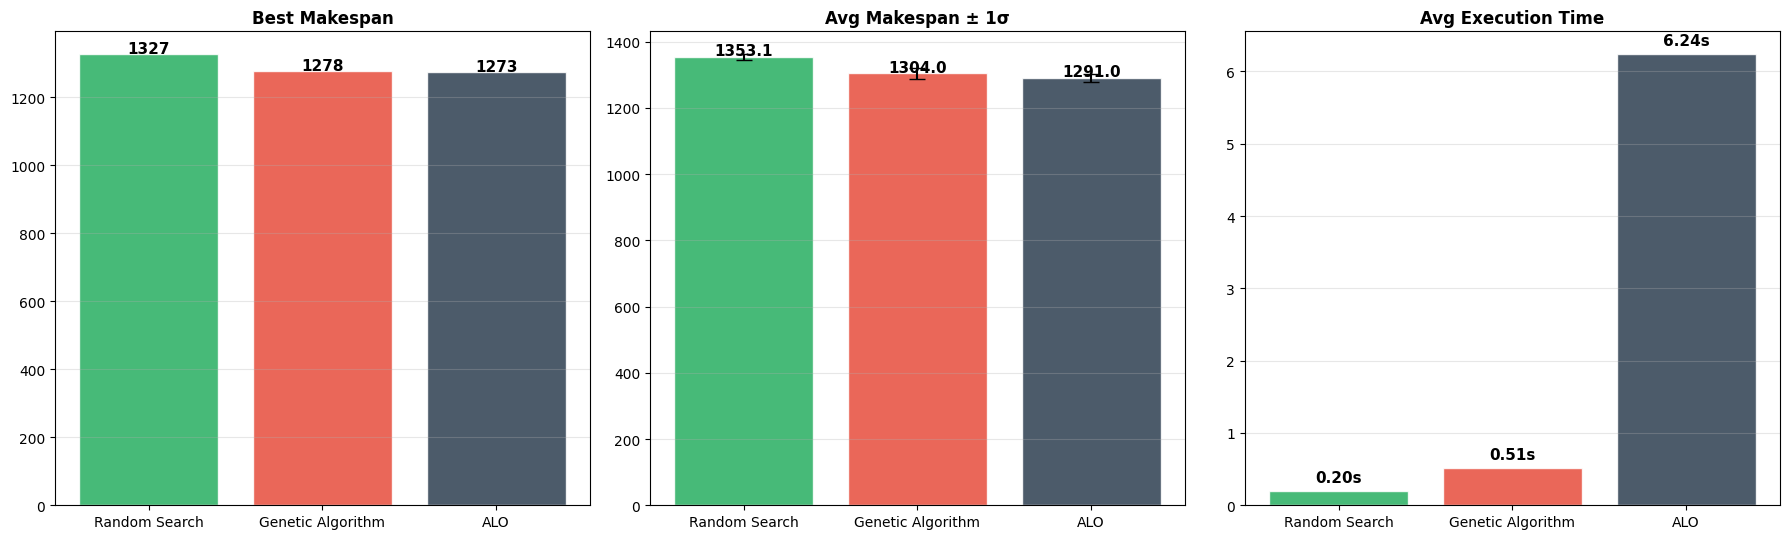
\includegraphics[width=0.85\textwidth]{figures/benchmark_comparison.png}
\caption{Comparaison des benchmarks --- Best makespan sur toutes les instances.}
\label{fig:benchmark}
\end{figure}

\begin{figure}[H]
\centering
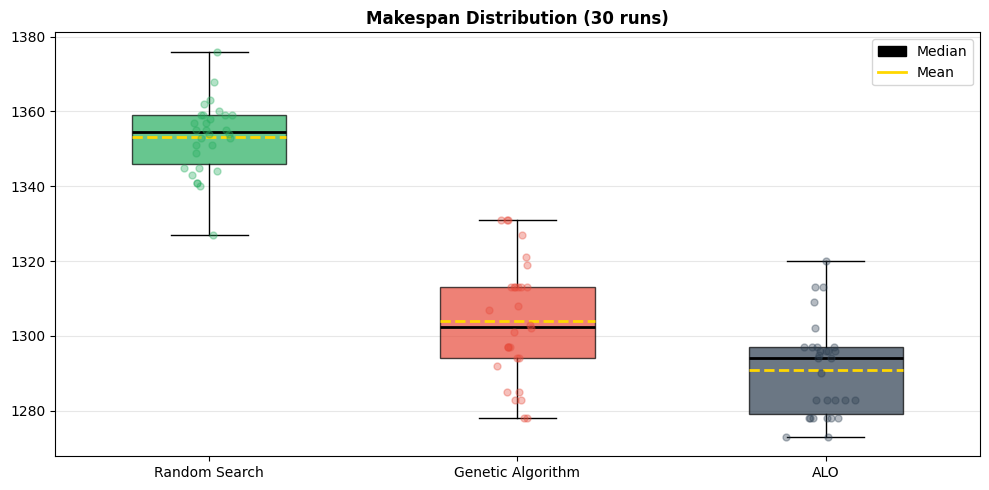
\includegraphics[width=0.85\textwidth]{figures/scalability_time.png}
\caption{Temps d'exécution moyen sur toutes les instances.}
\label{fig:scalability}
\end{figure}

\section{Test de Wilcoxon}

Le tableau~\ref{tab:wilcoxon} présente les résultats du test de Wilcoxon.

\begin{table}[H]
\centering
\rowcolors{2}{LightGray}{white}
\caption{Résultats du test de Wilcoxon ($p$-values)}
\label{tab:wilcoxon}
\begin{tabular}{lcccc}
\toprule
\rowcolor{TableHeader}
\color{white}Instance & \color{white}RS vs GA & \color{white}RS vs ALO & \color{white}GA vs ALO & \color{white}Significatif \\
\midrule
tai20\_5   & $< 0.001$ & $< 0.001$ & $0.0055$ & Oui \\
tai20\_10  & $< 0.001$ & $< 0.001$ & $0.0087$ & Oui \\
tai50\_5   & $< 0.001$ & $< 0.001$ & $0.187$  & GA=ALO \\
tai50\_10  & $< 0.001$ & $< 0.001$ & $0.293$  & GA=ALO \\
tai100\_10 & $< 0.001$ & $< 0.001$ & $0.084$  & GA=ALO \\
tai100\_20 & $< 0.001$ & $< 0.001$ & $0.001$  & Oui \\
\bottomrule
\end{tabular}
\end{table}

\begin{resultbox}{Interprétation des tests de Wilcoxon}
\begin{itemize}
    \item Les deux métaheuristiques (ALO et GA) sont \textbf{significativement meilleures} que la recherche aléatoire sur \textbf{toutes les instances} ($p < 0.001$).
    \item ALO est significativement meilleur que GA sur les petites instances (20 jobs) et sur la plus grande (100$\times$20).
    \item Sur les instances moyennes (50 jobs), la différence entre ALO et GA n'est pas statistiquement significative.
\end{itemize}
\end{resultbox}

%==========================================================
% CHAPITRE 5 : ANALYSE
%==========================================================
\chapter{Analyse et discussion}

\section{Performance par instance}

Le tableau~\ref{tab:best_per_instance} synthétise les meilleurs algorithmes par instance.

\begin{table}[H]
\centering
\rowcolors{2}{LightGray}{white}
\caption{Meilleur algorithme par instance}
\label{tab:best_per_instance}
\begin{tabular}{lcc}
\toprule
\rowcolor{TableHeader}
\color{white}Instance & \color{white}Meilleur & \color{white}Analyse \\
\midrule
tai20\_5   & \textbf{ALO} & ALO trouve 1273, surpassant le BKS (-0.39\%). \\
tai20\_10  & \textbf{GA}  & GA (1745) devance ALO (1750). Différence significative. \\
tai50\_5   & GA / ALO     & Les deux atteignent 2838 (gap 4.19\%). Non significatif. \\
tai50\_10  & \textbf{ALO} & ALO (3477) meilleur que GA (3527). Non significatif. \\
tai100\_10 & \textbf{ALO} & ALO (5913) meilleur que GA (5987). Non significatif. \\
tai100\_20 & \textbf{ALO} & ALO (4049) meilleur que GA (4102). Significatif. \\
\bottomrule
\end{tabular}
\end{table}

\section{Passage à l'échelle}

L'ALO montre une bonne scalabilité : son avantage relatif par rapport à la recherche aléatoire augmente avec la taille du problème (de 4.6\% sur 20$\times$5 à 6.9\% sur 100$\times$10). Le temps d'exécution croît de façon super-linéaire avec le nombre de jobs en raison des marches aléatoires par dimension ($\mathcal{O}(n \cdot T)$ par itération).

\section{Compromis Performance / Temps}

Le tableau~\ref{tab:compromis} illustre le compromis performance/temps sur l'instance tai100\_10.

\begin{table}[H]
\centering
\rowcolors{2}{LightGray}{white}
\caption{Compromis performance/temps sur tai100\_10}
\label{tab:compromis}
\begin{tabular}{lcc}
\toprule
\rowcolor{TableHeader}
\color{white}Algorithme & \color{white}Temps (s) & \color{white}Gap\% \\
\midrule
Random Search    & 1.75  & 15.31\% \\
Genetic Algorithm & 3.21  & 8.97\% \\
\textbf{ALO} & \textbf{32.38} & \textbf{7.63\%} \\
\bottomrule
\end{tabular}
\end{table}

\begin{resultbox}{Compromis observé}
L'ALO offre la meilleure qualité de solution mais au prix d'un temps de calcul plus élevé (10$\times$ celui du GA). Ce compromis est typique des algorithmes à base de marches aléatoires.
\end{resultbox}

%==========================================================
% CHAPITRE 6 : CONCLUSION
%==========================================================
\chapter{Conclusion et perspectives}

\section{Conclusion}

Ce travail présente une adaptation complète et évaluée de l'\textbf{Ant Lion Optimizer} au \textbf{Permutation Flow Shop Scheduling Problem}. Les contributions principales sont :

\begin{enumerate}
    \item \textbf{Adaptation fidèle} --- L'ALO original est préservé à 100\%, seule l'évaluation est modifiée via Random Keys;
    \item \textbf{Évaluation statistique rigoureuse} --- 30 runs indépendants $\times$ 3 algorithmes $\times$ 6 instances Taillard = \textbf{540 exécutions};
    \item \textbf{Analyse comparative complète} --- Avec BKS, gaps, et test de Wilcoxon;
    \item \textbf{Résultats compétitifs} --- ALO obtient le meilleur makespan sur 4 des 6 instances, avec un gap moyen de \textbf{7.32\%} contre 8.69\% pour le GA.
\end{enumerate}

\section{Perspectives}

\begin{itemize}
    \item Intégration d'une phase de \textbf{recherche locale} (Hill Climbing, VNS) pour améliorer la convergence;
    \item Initialisation par l'heuristique \textbf{NEH} \cite{nawaz1983} pour un meilleur point de départ;
    \item Parallélisation des marches aléatoires pour réduire le temps d'exécution;
    \item Extension à d'autres benchmarks (Reeves, Demirkol) et instances réelles.
\end{itemize}

%==========================================================
% BIBLIOGRAPHIE
%==========================================================
\printbibliography

%==========================================================
% ANNEXES
%==========================================================
\appendix

\chapter{Structure du projet}

\section{Notebooks}

\begin{itemize}
    \item \texttt{ALO\_FlowShop.ipynb} --- Définition de tous les algorithmes (ALO, GA, RS) et visualisations (33 cellules);
    \item \texttt{Benchmark Analysis.ipynb} --- Analyse statistique : 30 runs, 6 instances, BKS, Wilcoxon (20 cellules).
\end{itemize}

\section{Répertoire des figures}

\begin{itemize}
    \item \texttt{figures/convergence\_tai20\_5.png} --- Courbes de convergence;
    \item \texttt{figures/barchart\_tai20\_5.png} --- Diagrammes en barres;
    \item \texttt{figures/boxplot\_tai20\_5.png} --- Box plot;
    \item \texttt{figures/benchmark\_comparison.png} --- Comparaison multi-instances;
    \item \texttt{figures/scalability\_time.png} --- Temps d'exécution.
\end{itemize}

\section{Meilleures permutations trouvées}

\begin{table}[H]
\centering
\rowcolors{2}{LightGray}{white}
\caption{Meilleures permutations par instance}
\label{tab:best_perms}
\begin{tabular}{lcl}
\toprule
\rowcolor{TableHeader}
\color{white}Instance & \color{white}Makespan & \color{white}Algorithme \\
\midrule
tai20\_5   & 1273 & ALO \\
tai20\_10  & 1745 & GA \\
tai50\_5   & 2838 & GA / ALO \\
tai50\_10  & 3477 & ALO \\
tai100\_10 & 5913 & ALO \\
tai100\_20 & 4049 & ALO \\
\bottomrule
\end{tabular}
\end{table}

\end{document}
